\begin{frame}{Acceptance --- $K^{0}$ rejection effect}
  
  \begin{tabular}{cc}
    \begin{minipage}{0.5\hsize}
      \begin{figure}
        $d(K^-, n)"\pi^-\Sigma^+"$ \\
        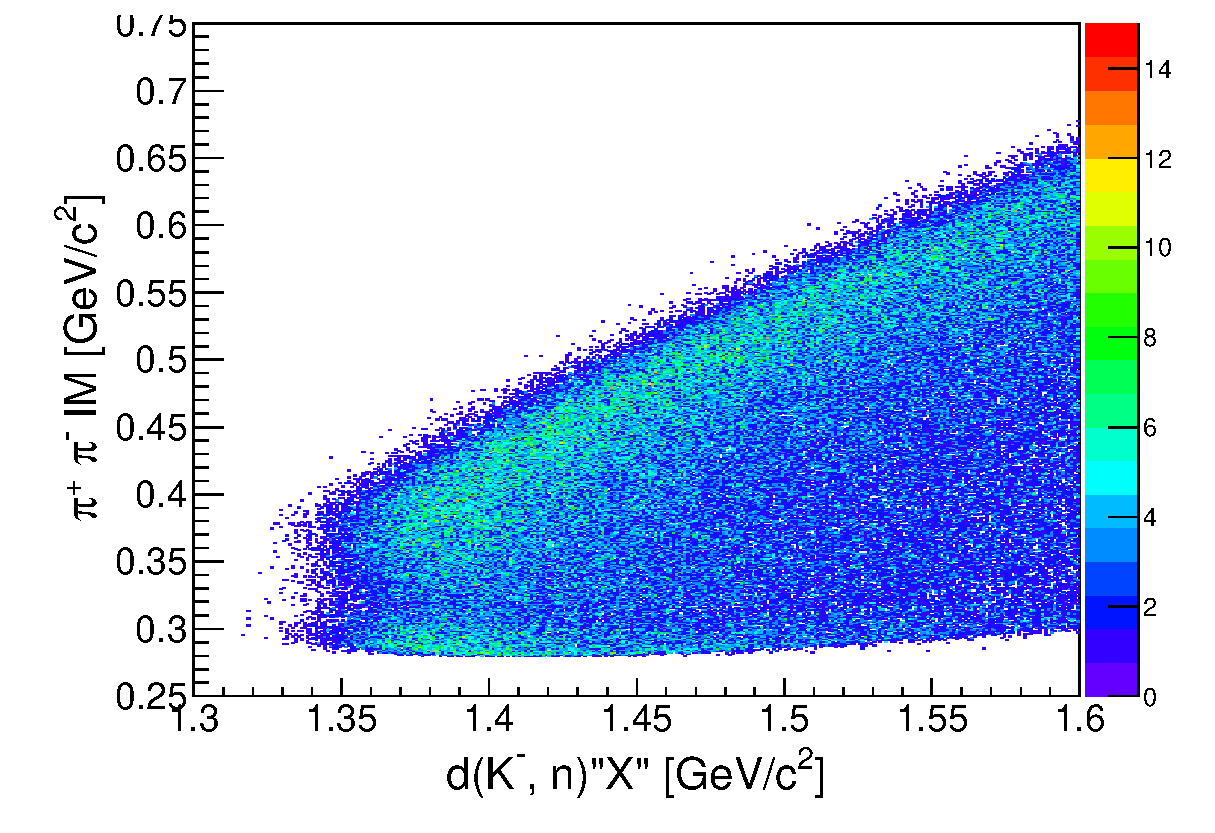
\includegraphics[width=4.5cm]{../pic/Run78/KN_ana/KN_MM_IM_pipi_pimSp.eps}
        \includegraphics[width=4.5cm]{../pic/Run78/KN_ana/acc_pipSm_cutK0.eps}
      \end{figure}
    \end{minipage}
    
    \begin{minipage}{0.5\hsize}
      \begin{figure}
        $d(K^-, n)"\pi^+\Sigma^-"$ \\
        \includegraphics[width=4.5cm]{../pic/Run78/KN_ana/KN_MM_IM_pipi_pipSm.eps}
        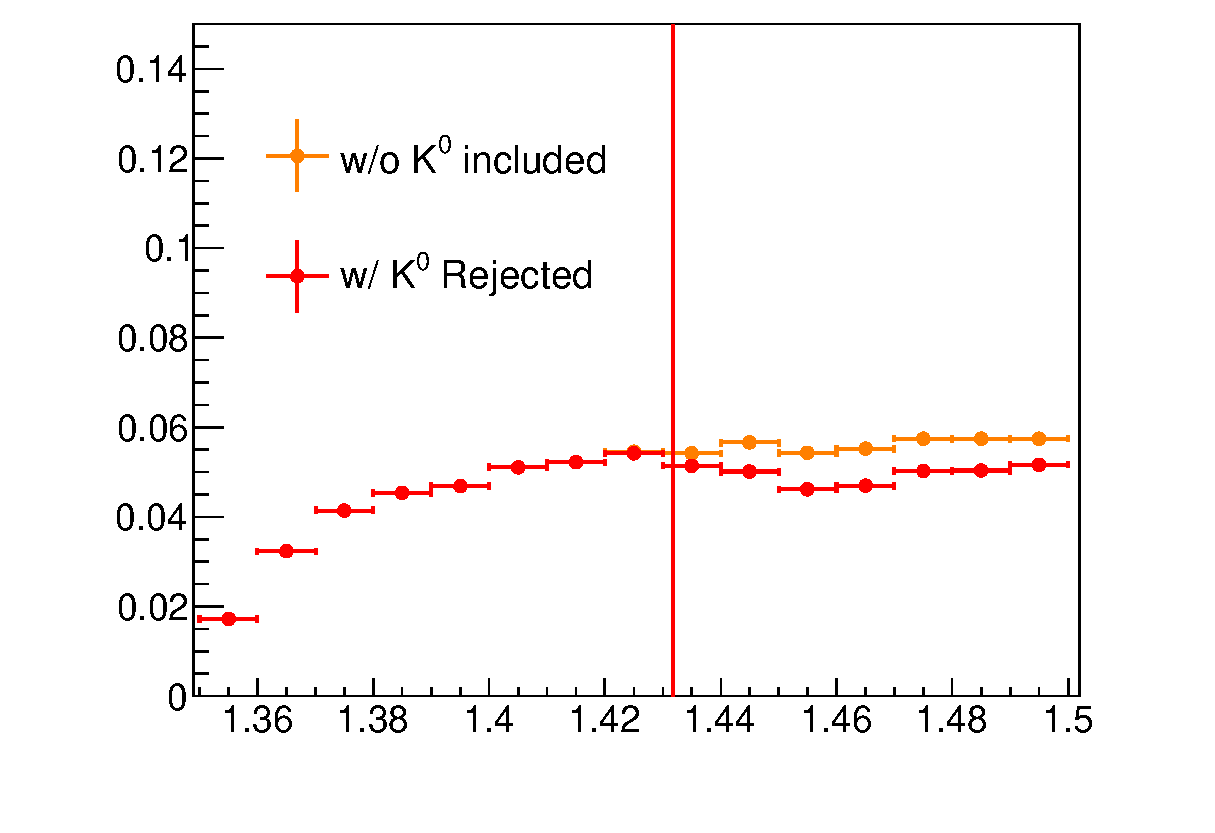
\includegraphics[width=4.5cm]{../pic/Run78/KN_ana/acc_pimSp_cutK0.eps}
      \end{figure}
    \end{minipage}
  \end{tabular}
  \centering
  $K^0$の除去は$\bar{K}N$閾値以上の部分に影響がある。
%%  上図は$d(K^-, n \pi^+ \pi^-)"n"$ selection入れていない
\end{frame}
